\documentclass[
12pt,
a4paper,
twoside,
openright
]{report}

% --- packages ---
\usepackage[
top=2cm,
bottom=2.6cm,
inner=3.5cm,
outer=2.5cm
]{geometry}
\usepackage[ngerman]{babel}
\usepackage[T1]{fontenc}
\usepackage[utf8]{inputenc}
\usepackage{setspace}
\usepackage{emptypage}
\usepackage{graphicx}
\usepackage{tikz}
\usepackage{amsmath, amssymb}
\usepackage{booktabs}
\usepackage{csquotes}
\usepackage{fontspec}
\setmainfont{Arial}
\usepackage{fancyhdr}
\usepackage[backend=biber,style=authoryear]{biblatex}
\usepackage{hyperref}

% bib
\addbibresource{quellen.bib}

%\setlength{\headheight}{14pt}
\setlength{\parindent}{0pt}
\setlength{\parskip}{6pt}


\pagestyle{fancy}
\fancyhf{}

\renewcommand{\headrulewidth}{0.5pt}

% Außen: Seitenzahl | Innen: Kapitel
\fancyhead[RO]{\thepage}
\fancyhead[LE]{\thepage}
\fancyhead[LO]{\nouppercase{\leftmark}}
\fancyhead[RE]{\nouppercase{\leftmark}}

% Kapitelmarke ohne "Kapitel X"
\renewcommand{\chaptermark}[1]{%
	\markboth{#1}{}%
}

\fancypagestyle{plain}{
	\fancyhf{}
	\renewcommand{\headrulewidth}{0.5pt}
	\fancyhead[RO]{\thepage}
	\fancyhead[LE]{\thepage}
	\fancyhead[LO]{\nouppercase{\leftmark}}
	\fancyhead[RE]{\nouppercase{\leftmark}}
}

\setstretch{1.4}

\begin{document}
	
	\thispagestyle{empty}

\begin{tikzpicture}[remember picture,overlay]
	
	\coordinate (TL) at (current page.north west);
	
	\node[anchor=north east] at ([xshift=-22mm,yshift=-11mm]current page.north east) {%
		
\includegraphics[width=55mm]{images/hsmw_logo.pdf}
	};
	
	\node[anchor=west] at ([xshift=35mm,yshift=-98mm]TL) {%
		{\fontsize{30pt}{14pt}\selectfont\bfseries BACHELORARBEIT}
	};
	
	\node[anchor=west,align=right, text width=98mm] at ([xshift=35mm,yshift=-160mm]TL) {
		{\fontsize{14pt}{14pt}\selectfont
		  Herr Paul Fuchs}	};
	
	\node[anchor=west,align=right,text width=98mm] at ([xshift=35mm,yshift=-200mm]TL) {%
		{\fontsize{16pt}{20pt}\selectfont
			Die Downtime-freie Bereitstellung von\\Microservices in Kubernetes Umgebungen.}
	};
	
	\node[anchor=west,align=right, text width=98mm] at ([xshift=35mm,yshift=-250mm]TL) {%
		{\fontsize{14pt}{14pt}\selectfont 2026}
	};
	
\end{tikzpicture}

\cleardoublepage

	
	\thispagestyle{empty}
	% Titelseite
	\begin{titlepage}	
		\raggedleft
		\vspace*{2cm}
		
		{\large Fakultät Angewandte Computer- und Biowissenschaften\par}
		
		\vspace{1cm}
		\hrule
		\vspace{0.5cm}
		{\huge \textbf{BACHELORARBEIT}\par}
		\vspace{0.5cm}
		\hrule
		\vspace{2cm}
		
		{\LARGE \textbf{Die Downtime-freie Bereitstellung von Microservices in Kubernetes Umgebungen.}\\[1.5cm]}
		\vfill
		\raggedleft
		\begin{tabular}{l}
			Autor: \\ \textbf {Paul Fuchs} \\ \\
			Seminargruppe: \\ MI20w2-B \\ \\
			Studiengang: \\ Medieninformatik und  \\ Interaktives Entertainment \\ \\
			Erstprüfer: \\ Prof. Philipp Klimant  \\ \\
			Zweitprüfer: \\ Dr. Beier-Grunwald \\ \\
			Einreichung: \\ Mittweida, den 27.03.2026
		\end{tabular}
	\end{titlepage}
	
	\cleardoublepage
	\subsubsection*{Bibliografische Angaben}
	Fuchs, Paul: Die Downtime-freie Bereitstellung von Microservices in Kubernetes Umgebungen. TODO:  5 Seiten, 14 Abbildungen, 1 Anlage mit Quelltexten, Hochschule Mittweida (FH), Fachbereich Angewandte Computer- und Biowissenschaften \\ \\
	Bachelorarbeit 2026
	\vfill 
	Abstract
	TODO 
	
	\pagenumbering{Roman}
	% Inhaltsverzeichnis
	
	\tableofcontents
	\listoffigures
	\listoftables
	
	\cleardoublepage
	
	\pagenumbering{arabic}
	
	% Einleitung
	\chapter{Einleitung}
	\section{Problemstellung}
	
	\section{Forschungsfrage}
	Wie verringern Canary Release mit Service Level Objective basierten Analysen den Verbrauch des Fehlerbudgets im Vergleich zu Rolling Updates mit Alertmanager?
	
	
	\chapter{Theoretische Grundlagen}
	
	\section{Microservice Architektur}
	
	\section{Microservice Orchestrierung mit Kubernetes}
	
	\section{Deployment Strategien}
	
	\section{Site Reliability Engineering und dessen Konzepte}
	
	\section{Monitoring und Observability}
	
	\chapter{Konzeption und Methodik}
	Als sinnbildliches Szenario wurde ein Online-Shop gewählt. Die Architektur des Systems besteht aus zwei Microservices, jeweils ein Repräsentant für den Shop und für die Transaktionen. Zwischen den Services besteht technisch keine Abhängigkeit. Im Microservice für die Transaktionen wird ein simulierter Fehler injiziert, während der Shop-Microservice als Referenz dient, um gegebenenfalls infrastrukturelle Fehler erkennbar zu machen, welche nicht auf die injizierten Fehler zurückzuführen sind. Da es sich hierbei um eine nutzerzentrierte Anwendung handelt, werden zwei Fehlerszenarien überprüft. Einerseits die Injektion einer Fehlerrate, in dem der Service einen internen Serverfehler produziert. Andererseits die Simulation verlängerter Antwortzeit. Es wurde jeweils überprüft, wie lange die jeweilige Analyse benötigt, den Fehler zu erkennen und anschließend den stabilen Zustand widerherzustellen. Weiter wurde berechnet, wie hoch der Verbrauch des Fehlerbudgets innerhalb des getesteten Zeitfensters war.
	
	\section{Systemarchitektur}
	Das System wurde in einem AWS EKS Cluster mit zwei m7i-flex.large Nodes aufgesetzt. Diese wurden jeweils dediziert für die Ausführung der Monitoring-Software und Lasttests und die Ausführung der zu testenden Services konfiguriert. Dies verhindert, dass die Messungen durch Konkurrenz um Hardware-Ressourcen beeinflusst werden. 
	Abbildung \ref{fig:system_arch} veranschaulicht diesen Zustand noch einmal tiefergehend. Hinzuzufügen ist bei der Systemarchitektur, dass Cilium als Service-Mesh konfiguriert wurde. Dies hätte das Monitoring für die Nutzung der Services von außerhalb des Clusters vereinfacht. Da die Lasttests jedoch über den Cluster-internen DNS aufgelöst wurden, spielt die Implementierung dessen hier keine weitere Rolle.  
	\begin{figure}[htbp]
		\centering
		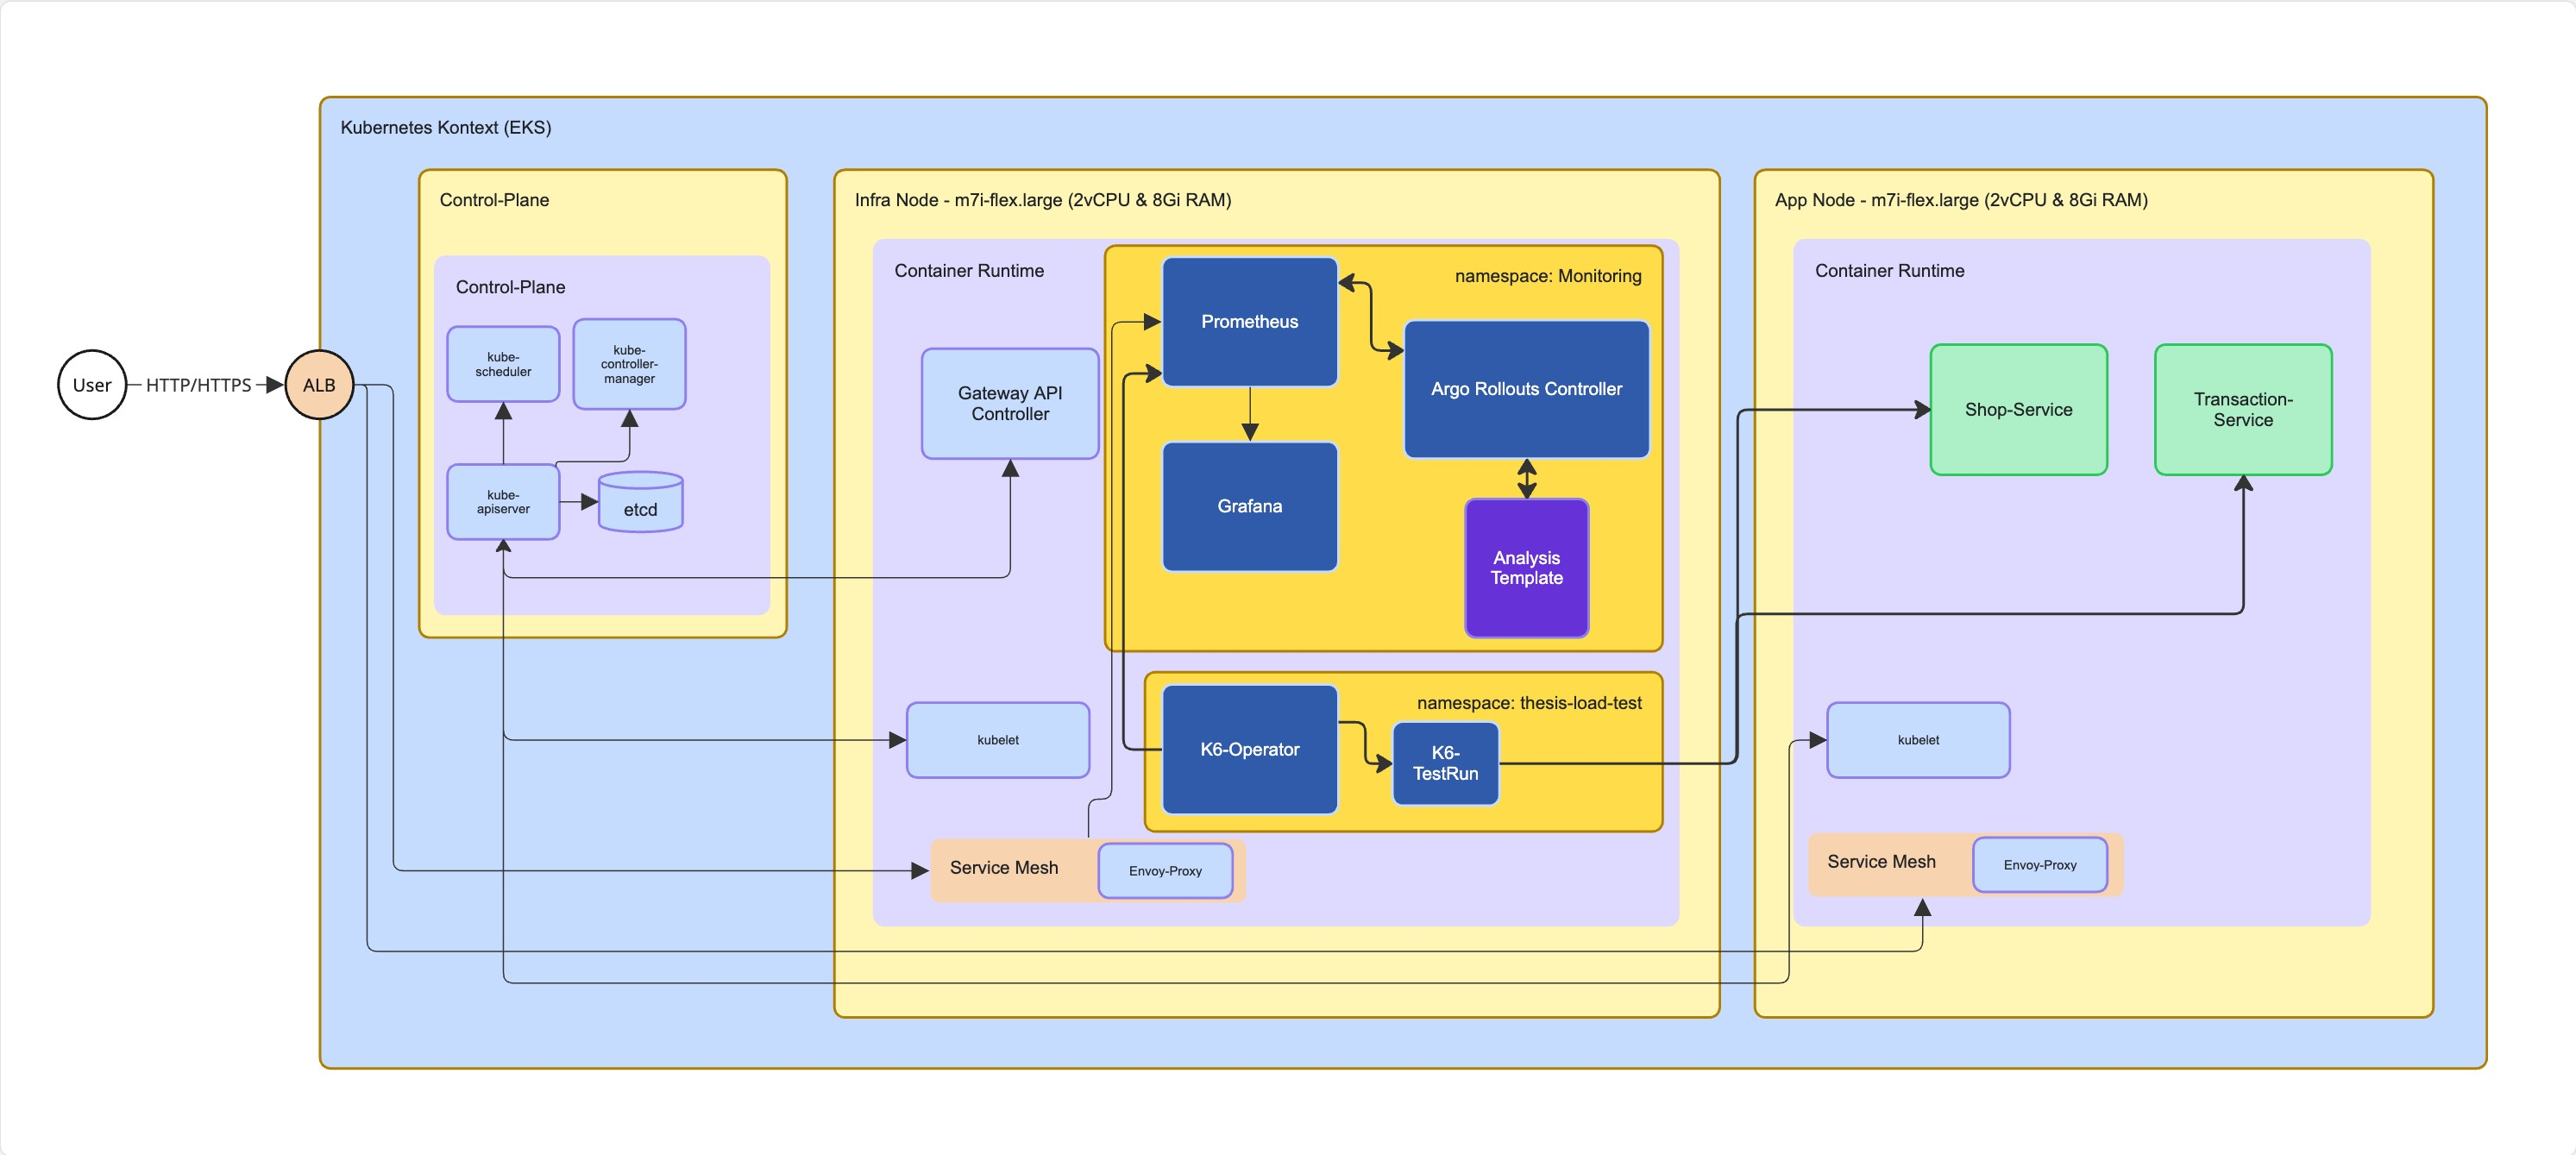
\includegraphics[width=0.8\textwidth]{images/sys-arch.jpg}
		\caption{Systemarchitektur: EKS Cluster Versuchsaufbau}
		\label{fig:system_arch}
	\end{figure} 
	Die zu testende Applikation besteht aus zwei JVM-basierten Microservices, welche sinnbildlich einen Online-Shop abbilden. Hierfür wurde als Server-Framework Ktor verwendet. Um Fehler während des Deployment Prozesses zu vermeiden, wurden die Container der Microservices jeweils mit Readiness-Probes und einer Mindest-Ready-Zeit von 20 Sekunden ausgestattet. Dies verhindert, dass die Services Anfragen an Pods weiterleten, die sich im Warmup-Prozess befinden. Weiter wurden die Container mit Pre-Stop Hooks von 20 Sekunden versehen, so wird verhindert, dass Anfragen an Pods geleitet werden, die bereits herunterfahren. Um die Erreichbarkeit der Pods sicherzustellen wurden Liveness-Probes implementiert. Diese Applikationen werden auf der Node mit dem Label \textit{role: app-node} gehostet. Die folgenden Software-Tools wurden so konfiguriert, dass sie auf der Node mit dem Label \textit{role: infra-node} ausgeführt werden. Um das Monitoring zu ermöglichen, wurden Prometheus und Grafana im Cluster deployed. Für die Implementierung der jeweiligen Deployment Strategie wurde Argo-Rollouts verwendet. Dies ermöglicht in Verbindung mit Prometheus die SLO-gesteuerte Analyse während des Deployment Vorgangs. Um die Nutzerlast auf den jeweiligen Service zu simulieren wurde K6 mit Constant-Arrival-Rate verwendet. Dies garantiert, dass die Services eine konstant gleichbleibende Last, unabhängig von der Antwortzeit bearbeiten müssen.
	
	\section{Theoretisches Modell}
	Rein mathematisch lässt sich bereits beweisen, dass Canary-Releases einen Vorteil beim Verbrauch des Fehlerbudgets gegenüber Rolling Updates haben, in dem Sinne, dass bei gleicher Art des Fehlers, Nutzer kontinuierlich gesteigerten Zugriff auf die neue Softwareversion erhalten. Genauer erklärt am Beispiel: Es wird ein Fehler in der Softwareversion ausgerollt, der in zwei Prozent aller Fälle einen Serverfehler verursacht. Für Rolling Updates erhalten während und nach der Bereitstellung alle Nutzer Zugang zu der neuen fehlerhaften Version, der Einfluss auf den Verbrauch des Fehlerbudgets spiegelt sich direkt wider. Bei Canary Updates werden während des Bereitstellungsprozesses kontinuierlich mehr Nutzer auf die fehlerhafte Version Zugriff erhalten, demnach spiegelt sich während des Deployment Prozesses der Einfluss auf den Verbrauch des Fehlerbudgets anteilig wider. Erst mit dem Abschluss des Canary Releases spiegelt sich der Einfluss direkt auf das Fehlerbudget wider. Weiter ist logisch herzuleiten, dass die Detektionszeit für den Fehler sinkt, wenn sich die Analyse auf die Canary-Version beschränkt, anstatt den Fehler im gesamten System zu überprüfen. Diese Arbeit analysiert den Faktor, um den die Detektionszeit und der Verbrauch des Fehlerbudgets, bei gleicher zeitlicher Analyseintervallrate zwischen Rolling Update und Canary Release mit globaler und isolierter Aggregation sinkt.
	
	\section{Parameter zur Analyse}
	Für die Erhebung der Daten wurden jeweils fünf Testläufe über 30 Minuten absolviert. Jeder Service war dabei einer Last von 1200 Anfragen pro Sekunde ausgesetzt. Die injizierten Fehler wurden mittels Umgebungsvariablen realisiert. Da Rolling Updates nativ keine Möglichkeit der Analyse bieten, habe ich mich dazu entschieden, das Alerting von Grafana zu verwenden. \\
	Für die Gewichtung des Datenverkehrs wurden folgende Schritte definiert, nach dem Erhöhen wurde das System für jeweils 5 Minuten überwacht, bevor der nächste Schritt erfolgte: 
	\begin{itemize}
		\item 10\% 
		\item 50\%
		\item 75\%
		\item 100\%
	\end{itemize}
	
	\subsection{Fehlerfreier Zustand des Systems}
	Der Zustand der Applikation wurde zuerst ohne injizierte Fehler analysiert, basierend darauf wurde die Definition der SLO's erstellt. Die für diese Arbeit wichtigen Definitionen umfassen: 
	\begin{itemize}
		\item eine Verfügbarkeit von 99\%
		\item eine Antwortzeit von 15ms für 95\% aller erfolgreichen Anfragen 
	\end{itemize}
	und beschreiben einen rollierenden Zeitraum von 30 Minuten, im Sinne der Testdauer.
	
	\subsection{Fehlerszenario A}
	In Fehlerszenario A wurde der Transaktions-Microservice so konfiguriert, dass er bei der Beantwortung einer Anfrage in 5\% der Fälle einen internen Serverfehler meldete. Die zu überprüfende Metrik im Hinblick auf das SLO, ist das Verhältnis fehlerhafter beantworteter Anfragen zur Summe aller Anfragen.
	
	\subsection{Fehlerszenario B}
	In Fehlerszenario B wurde der Transaktions-Microservice so konfiguriert, dass er bei der Beantwortung einer Anfrage zusätzlich zur normalen Antwortzeit 15ms warten musste. Die zu überprüfende Metrik ist die Antwortzeit über 95\% aller Anfragen, die ohne Fehler beantwortet wurden.
	
	\subsection{Analyseintervalle}
	Um ein einheitliches Analyse-Verfahren zu garantieren, wurden die Werte für die Analyseintervalle für alle Analysemethoden vereinheitlicht. Alle 60 Sekunden findet die Überprüfung der Metrik statt. Während für die Analysistemplates ein Fehlerlimit von eins gesetzt wurde, was eine einmalige Überschreitung des Schwellwerts zulässt, wurde der Alertmanager genauso konfiguriert, sodass er bei der ersten Schwellwertüberschreitung den Pending Status annimmt, demnach zulässt und erst bei der zweiten Schwellwertüberschreitung den alarmierten Zustand auslöst.
	
	\chapter{Evaluation}
	Für die Fehlerszenarien wurden die Zeit bis zur Detektion und die Zeit bis zur Wiederherstellung des stabilen Zustands mithilfe der Kubernetes Events bestimmt. Weiter werden die einzelnen Testläufe im zeitlichen Verlauf nebeneinander dargestellt und abschließend werden die gemittelten Werte der unterschiedlichen Deployment Strategien im Kombinationsdiagramm miteinander verglichen.
	
	\section{Analyse der injizierten Fehlerrate}
	\subsection{Mittlere Detektionszeit und Mittlere Wiederherstellungszeit}
	Abbildung \ref{fig:mttd-mttr-error} zeigt, dass die Zeit bis zur Detektion für Rolling Updates im Vergleich zu den Canary Methoden mit rund 3,3 Minuten am geringsten war. Gefolgt von der Canary Methode mit isolierter Metrikanalyse mit rund 8 Minuten, am längsten benötigte die Canary Methode mit globaler Analysemetrik, hier betrug die Zeit bis zur Detektion im Schnitt 12 Minuten. Die geringste Wiederherstellungszeit erreichte die Canary Methode mit isolierter Metrikanalyse, im Durchschnitt betrug die Zeit rund eine halbe Minute. Die zeitlichen Unterschiede lassen sich mit dem Versuchsaufbau erklären. Bei den Rolling Updates wurde der Fehler sofort erkennbar, da 5\% aller Anfragen an das System fehlschlugen. Der zeitliche Unterschied zwischen den Canary Release Methoden lässt sich mit der verwendeten Analysemetrik begründen. Für die globale Aggregation musste die Gewichtung des Datenverkehrs erst einen signifikanten Schwellwert überschreiten, dass die Fehler nicht von den fehlerfreien Pods überlagert wurden. Die isolierte Analyse stellte hingegen das direkte Verhältnis der fehlerhaften Anfragen zu den Gesamtanfragen an die Canary Version gegenüber und konnte daher einen zeitlichen Vorteil erlangen. Diskutiert wird später dennoch, weshalb während der initialen 10\% Gewichtung keine Fehler erkannt wurden, obwohl diese mathematisch Vorkommen sollten.
	Die Canary Methode mit globaler Analysemetrik stellte den stabilen Zustand innerhalb von rund einer Minute wieder her. Das Rolling Update benötigte für die Wiederherstellung des stabilen Zustands fast zwei Minuten. Die Wiederherstellungszeiten lassen sich in Zusammenhang mit der Anzahl an Pods bringen, die ausgetauscht werden mussten, um die fehlerfreie Version wieder lauffähig zu machen. Die Rolling Updates mussten der Reihe nach alle Pods ersetzen, während bei den Canary Release Methoden noch fehlerfreie Pods lauffähig waren. Der Zeitunterschied von isolierter und globaler Analysemetrik lässt sich weiter in Zusammenhang mit den fehlerfrei laufenden Pods bringen. Die Canary Methode mit isolierter Metrikanalyse detektierte die Fehler im zweiten Schritt, hier waren 50\% User-Traffic auf die neue Version umgeleitet und die fehlerfreie Pod Anzahl betrug zwei. Die Canary Methode mit globaler Analysemetrik detektierte den Fehler erst im dritten Schritt mit 75\% User-Traffic, die fehlerfreie Pod Anzahl betrug eins.
	
	\begin{figure}[htbp]
		\centering
		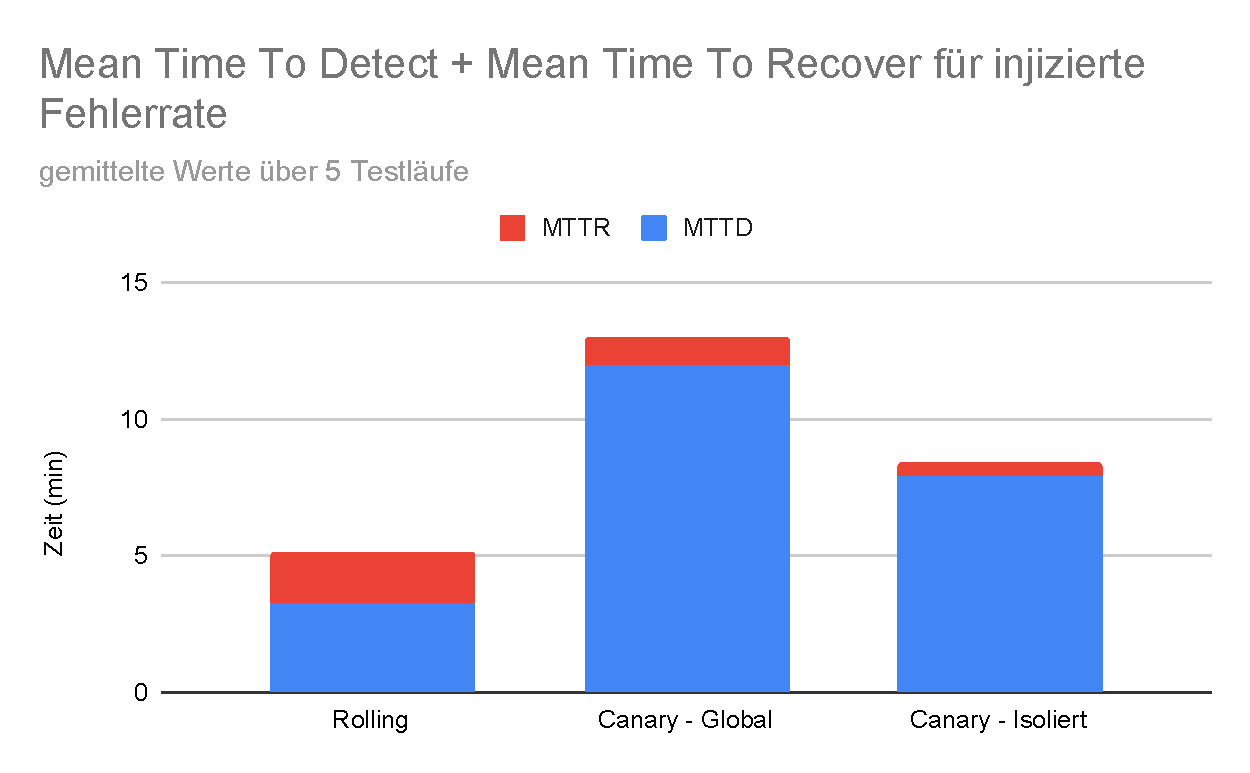
\includegraphics[width=0.8\textwidth]{images/eval-pdf/Mean Time To Detect + Mean Time To Recover für injizierte Fehlerrate.pdf}
		\caption{Summe der Zeit bis zur Detektion und der Zeit bis zur Wiederherstellung für injizierte Fehlerrate}
		\label{fig:mttd-mttr-error}
	\end{figure} 
	
	\subsection{Die einzelnen Testläufe im zeitlichen Verlauf}
	Die Diagramme zeigen den globalen Einfluss der injizierten Fehlerrate auf das System.
	Beginnend mit dem Vergleich der einzelnen Testläufe für das Rolling Update zeigt Abbildung \ref{fig:singles-rolling-error}, dass die Fehlerrate den Maximalwert von 5\% innerhalb von 5 Minuten erreichte und dieser nach Abschluss des Rollbacks wieder auf null sank. 
	
	\begin{figure}[htbp]
		\centering
		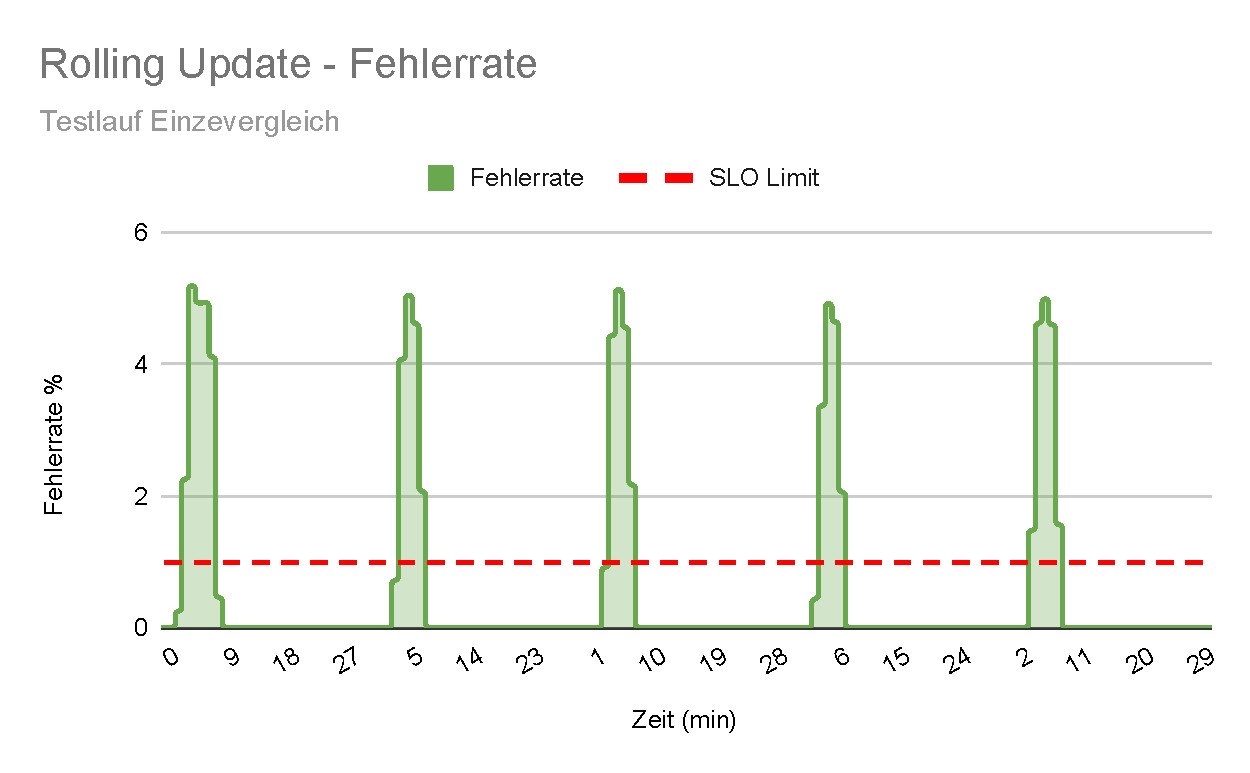
\includegraphics[width=0.8\textwidth]{images/eval-pdf/Rolling Update - Fehlerrate.pdf}
		\caption{Fehlerrate Rolling Update im Einzelvergleich}
		\label{fig:singles-rolling-error}
	\end{figure}
	
	In Abbildung \ref{fig:singles-canary-g-error} wird ersichtlich, dass die Canary Release Strategie mit globaler Metrikanalyse einen Maximalwert von 2,3\% Fehlerrate innerhalb von 13 Minuten erreichte. Auffällig ist der erste Testlauf, der nach elf Minuten seinen Peak von 1,1\% Fehlerrate erreichte und im Gegensatz zu den folgenden Testläufen direkt zurückgerollt wurde. Inwiefern die Analyse hier schneller reagiert, wird später diskutiert.
	
	\begin{figure}[htbp]
		\centering
		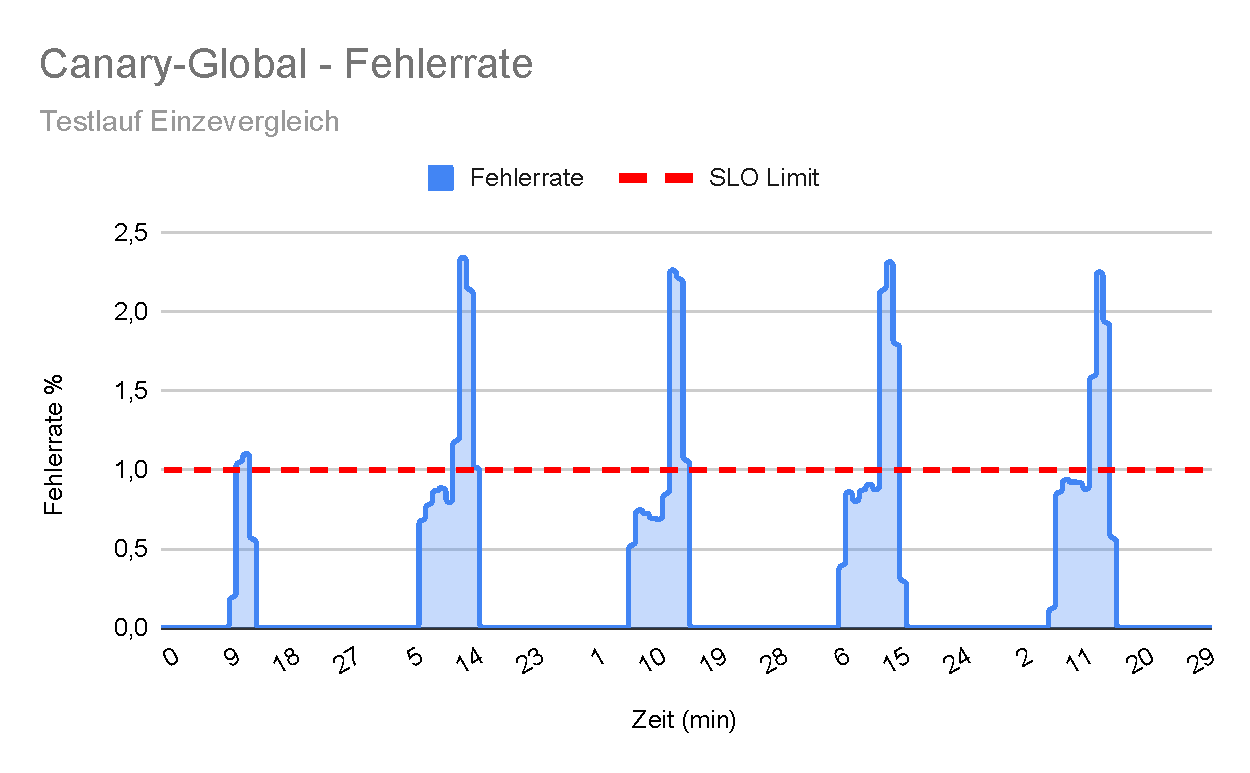
\includegraphics[width=0.8\textwidth]{images/eval-pdf/Canary-Global - Fehlerrate.pdf}
		\caption{Fehlerrate Canary Release globaler Metrikanalyse im Einzelvergleich}
		\label{fig:singles-canary-g-error}
	\end{figure} 
	
	Während beide vorherigen Deployment Strategien das SLO-Limit überschritten, zeigt Abbildung \ref{fig:singles-canary-i-error}, dass die isolierte Analysemetrik  das SLO-Limit erfolgreich über alle Testläufe eingehalten hat. Hier wurden die Maximalwerte im Schnitt innerhalb von neun Minuten erreicht.  
	
	\begin{figure}[htbp]
		\centering
		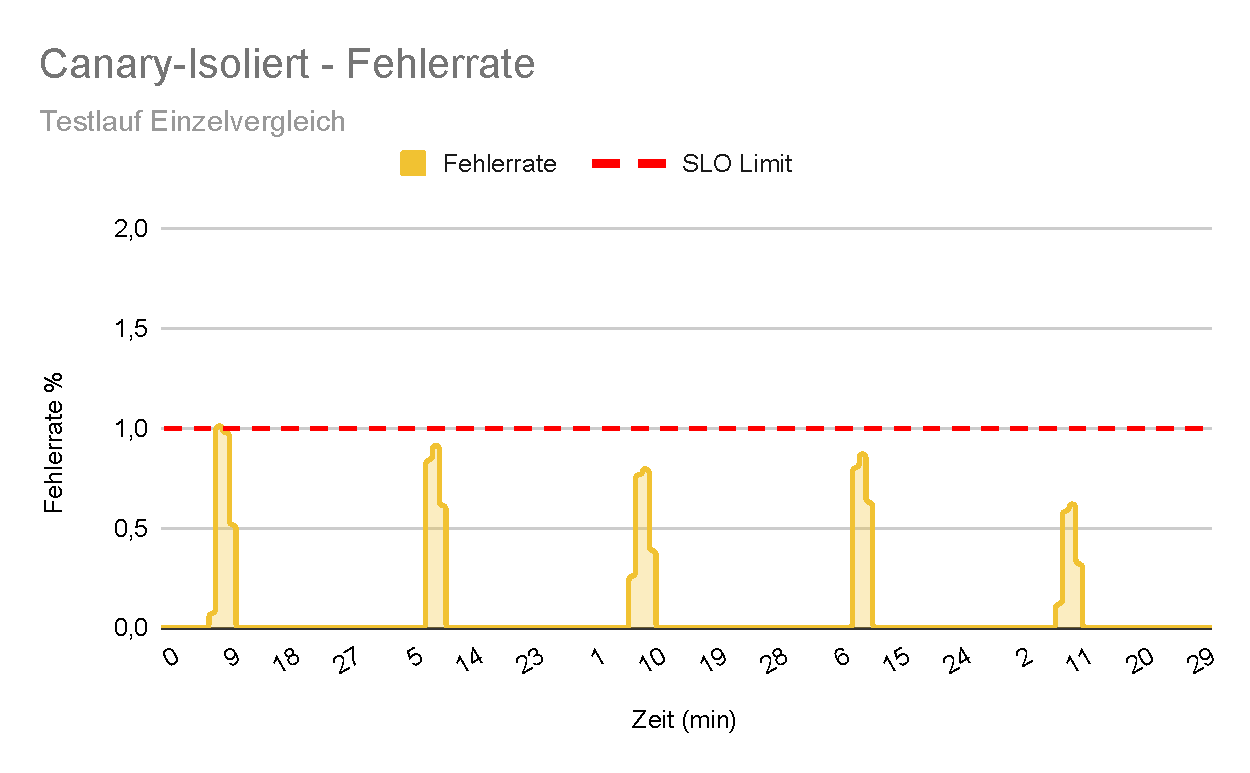
\includegraphics[width=0.8\textwidth]{images/eval-pdf/Canary-Isoliert - Fehlerrate.pdf}
		\caption{Fehlerrate Canary Release isolierter Analysemetrik im Einzelvergleich}
		\label{fig:singles-canary-i-error}
	\end{figure} 
	
	\subsection{Die gemittelten Werte der Deployment Strategien im Vergleich}
	Deutlicher werden die ermittelten Werte im direkten Vergleich der Deployment Strategien. In Abbildung \ref{fig:mid-error-by-strategy} wird der Zusammenhang aus Zeit bis zur Detektion und Einfluss der injizierten Fehlerrate für die unterschiedlichen Deployment Strategien stärker ersichtlich, als bei der Einzelbetrachtung. Während das Rolling Update bereits den Wiederherstellungsprozess der stabilen Version abgeschlossen hatte, entstanden die Fehler der Canary Methoden erst. Dafür begrenzte sich der Einfluss der injizierten Fehlerrate bei den Canary Methoden, während das Rolling Update die vollen 5\% injizierte Fehlerrate aufwies.
	
	\begin{figure}[htbp]
		\centering
		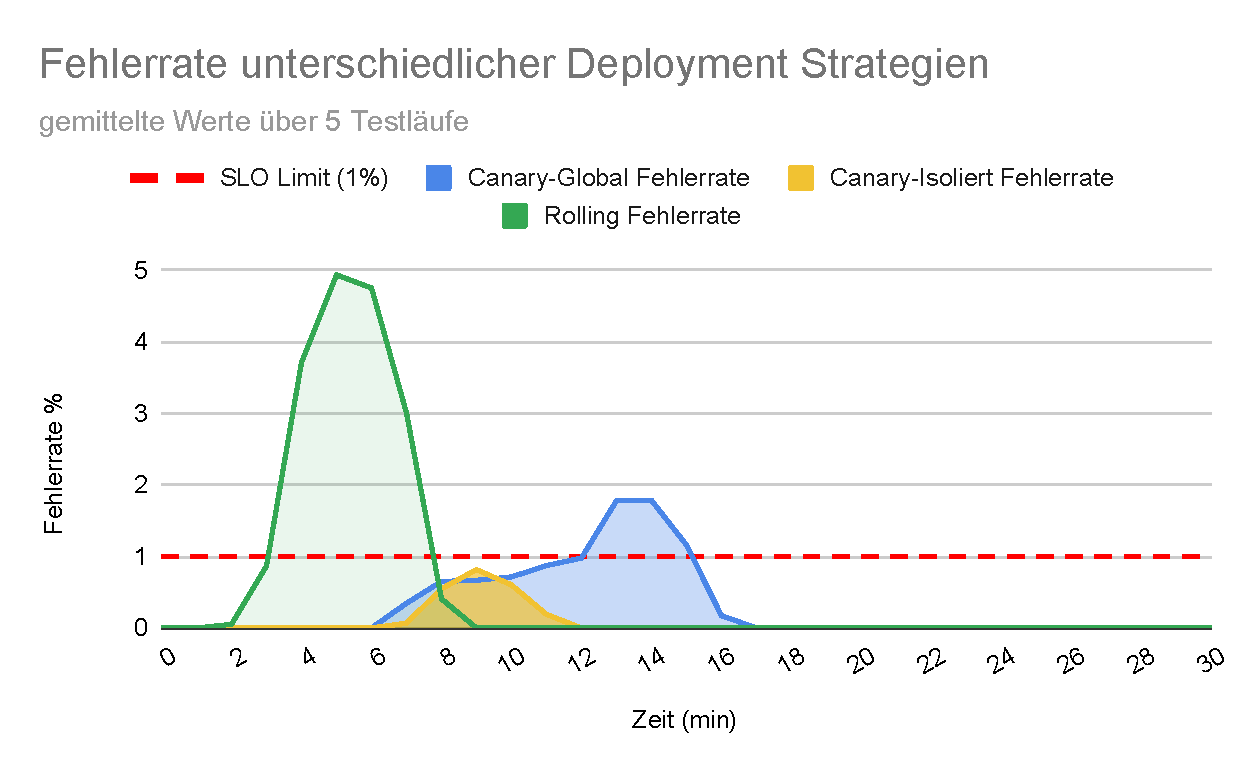
\includegraphics[width=0.8\textwidth]{images/eval-pdf/Fehlerrate unterschiedlicher Deployment Strategien.pdf}
		\caption{Fehlerrate unterschiedlicher Deployment Strategien}
		\label{fig:mid-error-by-strategy}
	\end{figure} 
	
	\section{Analyse der injizierten Latenz}
	\subsection{Mittlere Detektionszeit und Mittlere Wiederherstellungszeit}
	Abbildung \ref{fig:mttd-mttr-latenz} zeigt auch hier, dass das Rolling Update die geringste Zeit von der Fehlerinjektion bis zur Wiederherstellung des stabilen Zustands benötigte. Im Durchschnitt über alle Testläufe rund 6,9 Minuten. Das Canary Release mit isolierter Analysemetrik benötigte von der Injektion bis zur Wiederherstellung rund 7,3 Minuten, während das Canary Release mit globaler Metrikanalyse mit rund 13,3 Minuten am längsten benötigte. Wie auch im Fehlerszenario A lassen sich diese Zeiten mit dem direkten Einfluss des injizierten Fehlers für das Rolling Update erklären. Gleich gilt auch der Vorteil der isolierten Analyse der Canary Releases gegenüber dem globalen Ansatz, da für die isolierte Metrik, der direkte Einfluss der Canary Version überprüft wurde, hingegen musste bei der globalen Metrikanalyse erst eine ausreichend hohe Gewichtung des Datenverkehrs auf die Canary Version erreicht werden, damit der Fehler erkannt wurde.
	
	\begin{figure}[htbp]
		\centering
		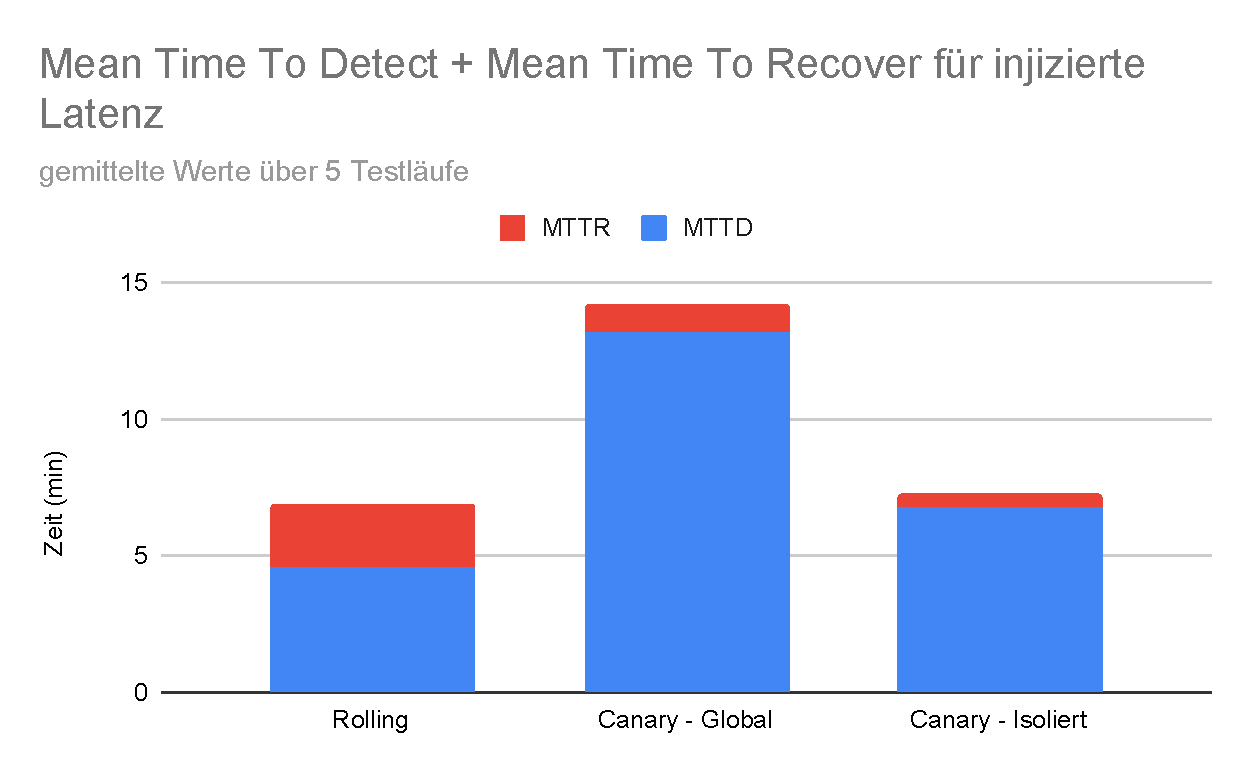
\includegraphics[width=0.8\textwidth]{images/eval-pdf/Mean Time To Detect + Mean Time To Recover für injizierte Latenz.pdf}
		\caption{Summe der Zeit bis zur Detektion und der Zeit bis zur Wiederherstellung für injizierte Latenz}
		\label{fig:mttd-mttr-latenz}
	\end{figure} 
	
	\subsection{Die einzelnen Testläufe im zeitlichen Verlauf}
	Die Diagramme zeigen den globalen Einfluss der injizierten Fehlerrate auf das System.
	Beginnend mit dem Vergleich der einzelnen Testläufe für das Rolling Update zeigt Abbildung \ref{fig:singles-rolling-latenz}, dass die Latenz Maximalwerte von über einer Sekunde Antwortzeit betrug. Dies ist mit blockierenden Threads zu erklären. Die Softwareversion hat es nicht geschafft die Anfragen in genügend geringer Zeit zu beantworten und die Pods wurden durch die Überlastung von CPU-Ressourcen kontinuierlich neu gestartet. Diese Unerreichbarkeit der Services ist als Downtime zu bewerten.
	
	\begin{figure}[h]
		\centering
		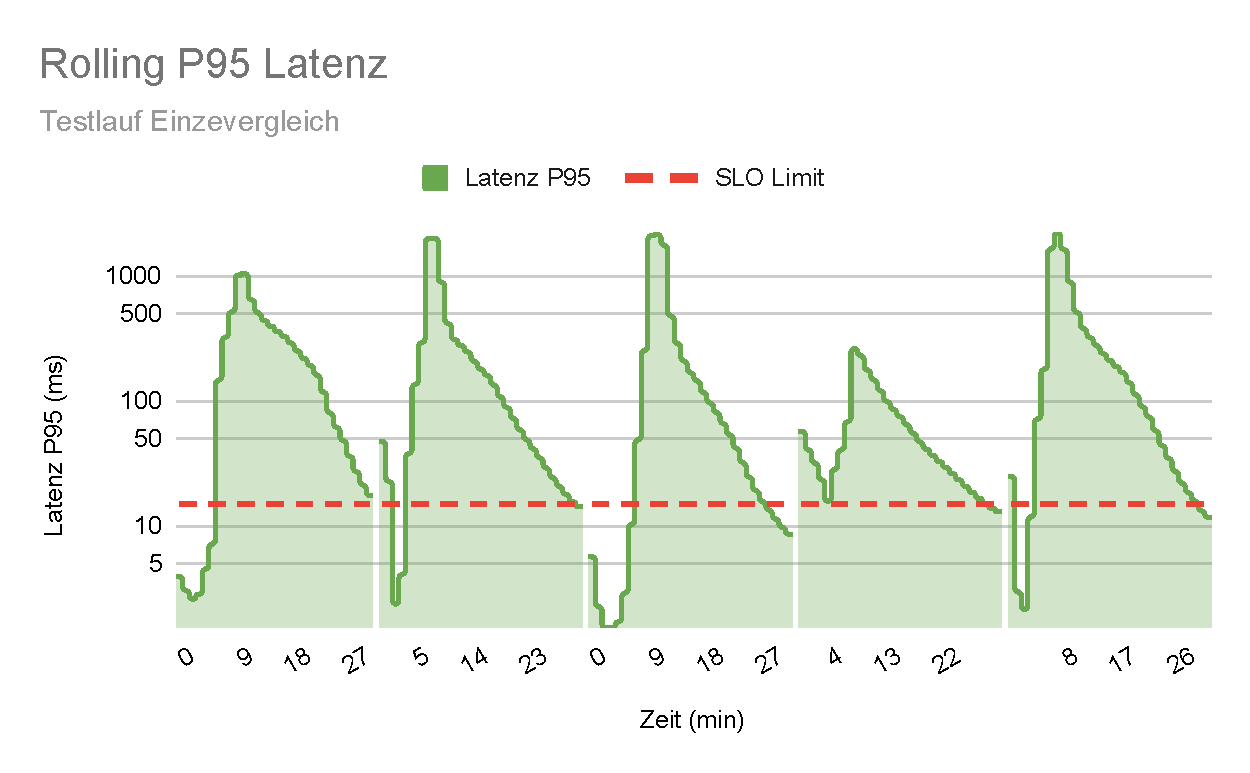
\includegraphics[width=0.8\textwidth]{images/eval-pdf/Rolling P95 Latenz.pdf}
		\caption{Latenz Rolling Update im Einzelvergleich}
		\label{fig:singles-rolling-latenz}
	\end{figure}
	
	In Abbildung \ref{fig:singles-canary-g-latenz} wird ersichtlich, dass die Canary Release Strategie mit globaler Metrikanalyse einen Maximalwert von bis zu 290 Millisekunden an Antwortzeit benötigte. Dies entspricht einer Steigerung um den Faktor 20 der erlaubten Antwortzeit entsprechend des SLO.
	
	\begin{figure}[htbp]
		\centering
		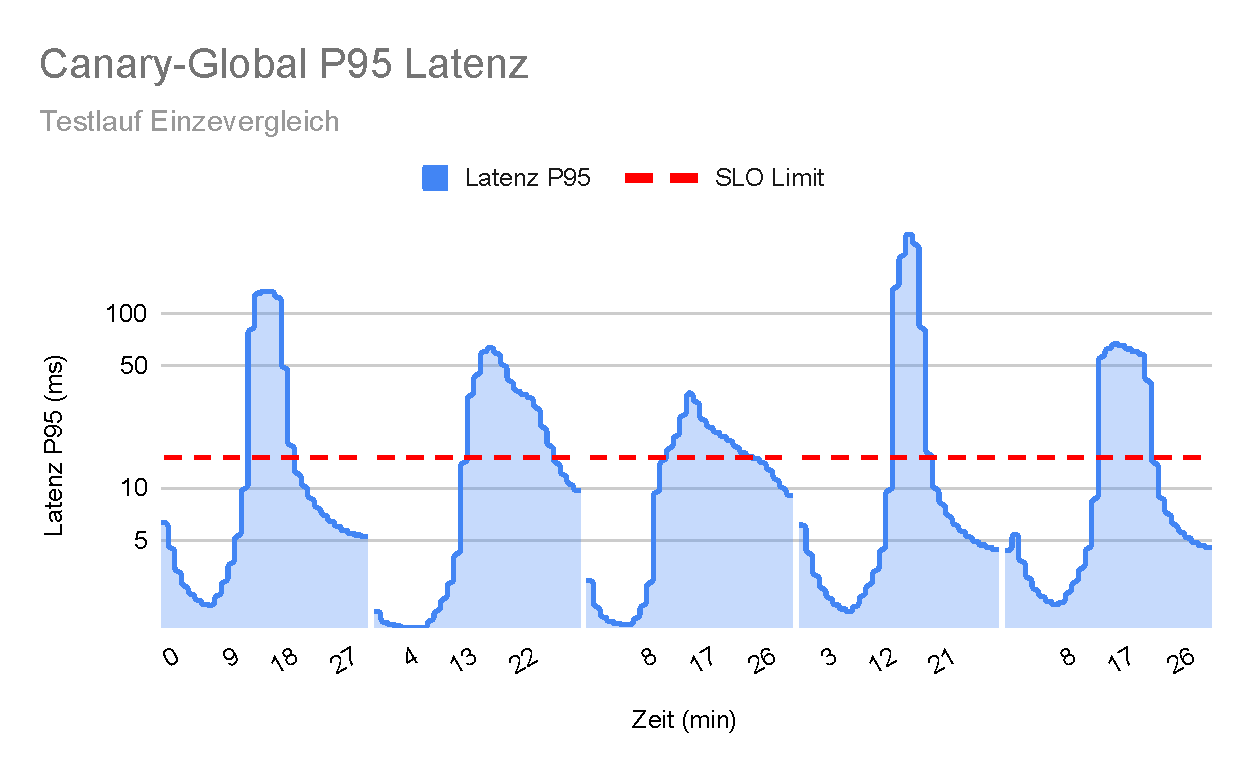
\includegraphics[width=0.8\textwidth]{images/eval-pdf/Canary-Global P95 Latenz.pdf}
		\caption{Latenz Canary Release globaler Metrikanalyse im Einzelvergleich}
		\label{fig:singles-canary-g-latenz}
	\end{figure} 
	
	Die beiden vorherigen Deployment Strategien überschritten das SLO-Limit deutlich, Abbildung \ref{fig:singles-canary-i-latenz} zeigt, dass die isolierte Analysemetrik  das SLO-Limit erfolgreich über alle Testläufe eingehalten hat. Auffällig sind im Diagramm einzig die Warm-Up Phasen während des Deploymentstarts.
	
	\begin{figure}[htbp]
		\centering
		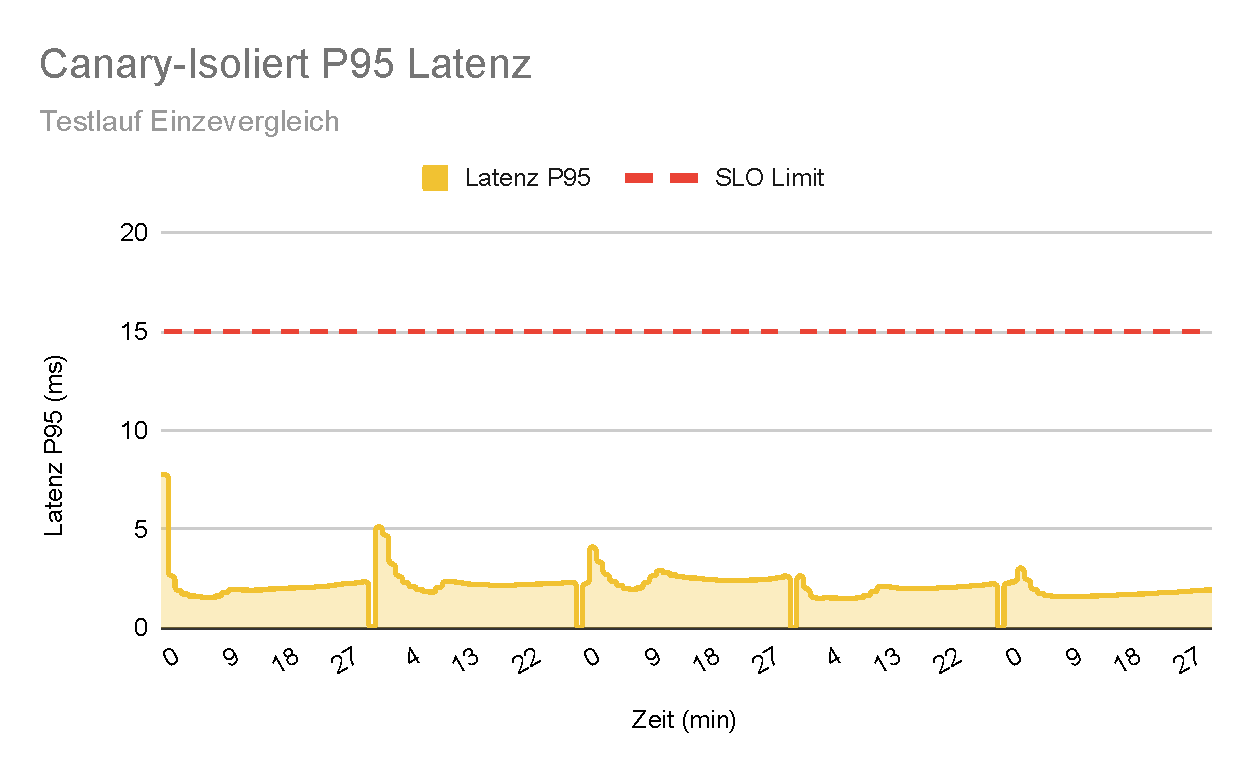
\includegraphics[width=0.8\textwidth]{images/eval-pdf/Canary-Isoliert P95 Latenz.pdf}
		\caption{Latenz Canary Release isolierter Analysemetrik im Einzelvergleich}
		\label{fig:singles-canary-i-latenz}
	\end{figure} 
	
	\subsection{Die gemittelten Werte der Deployment Strategien im Vergleich}
	Der direkte Vergleich der Deployment Strategien bringt die Überlegenheit des isolierten gegenüber des globalen Analyseansatzes und der Analyse des Rolling Updates deutlich zum Vorschein. Die globale Analyse des Canary Releases und das Rolling Update überschritten das gesetzte Limit bei Weitem. Während die isolierte Metrikanalyse des Canary Releases keinen Einfluss auf das Gesamtsystem aufweist.
	
	\begin{figure}[htbp]
		\centering
		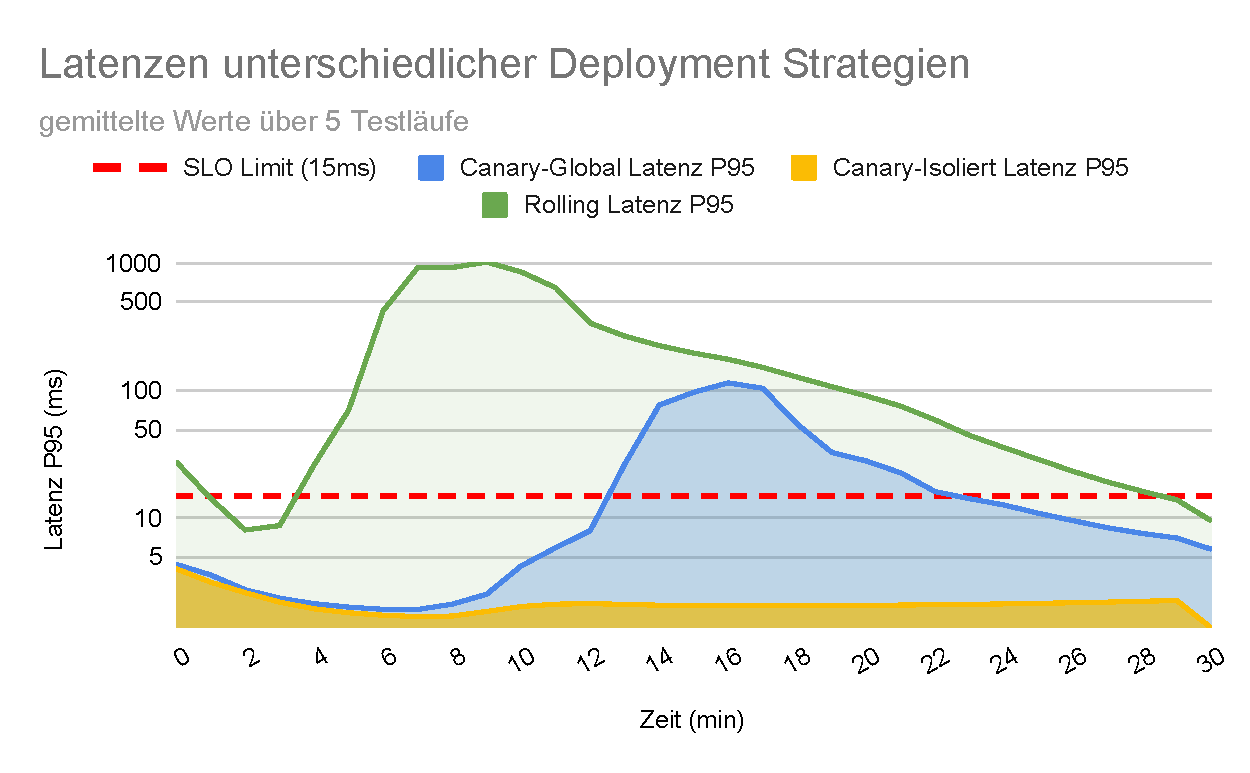
\includegraphics[width=0.8\textwidth]{images/eval-pdf/Latenzen unterschiedlicher Deployment Strategien.pdf}
		\caption{Latenzen unterschiedlicher Deployment Strategien}
		\label{fig:mid-latenz-by-strategy}
	\end{figure} 
	
	\section{Fehlerbudget Verbrauch pro Deployment Strategie}
	\subsection{Fehlerszenario A}
	Abbildung \ref{fig:mid-budget-consumption-error-by-strategy} zeigt den Einfluss der Analysemetrik und der Deployment Strategie auf den Verbrauch des Fehlerbudgets. Den geringsten Verbrauch erreichte die Canary Release Strategie mit isolierter Analyse. Der Bedarf betrug 7,4\% des Gesamtbudgets. Das Canary Release mit globaler Analyse erreichte einen Bedarf von 30,42\% am Gesamtbudget. Den höchsten Verbrauch des Fehlerbudgets bedurfte das Rolling Update mit 59,14\%. In diesem speziellen Szenario verringerte die Canary Release Strategie mit globaler Analysemetrik den Verbrauch des Fehlerbudgets im Gegensatz zum Rolling Update um 28,71 Prozentpunkte und die isolierte Analyse erreichte eine Verringerung des Budgetverbrauchs gegenüber dem Rolling um 51,72 Prozentpunkte. Weiter ist eine Verringerung des isolierten gegenüber dem globalen Ansatz um 23,01 Prozentpunkte festzuhalten.
	
	\begin{figure}[htbp]
		\centering
		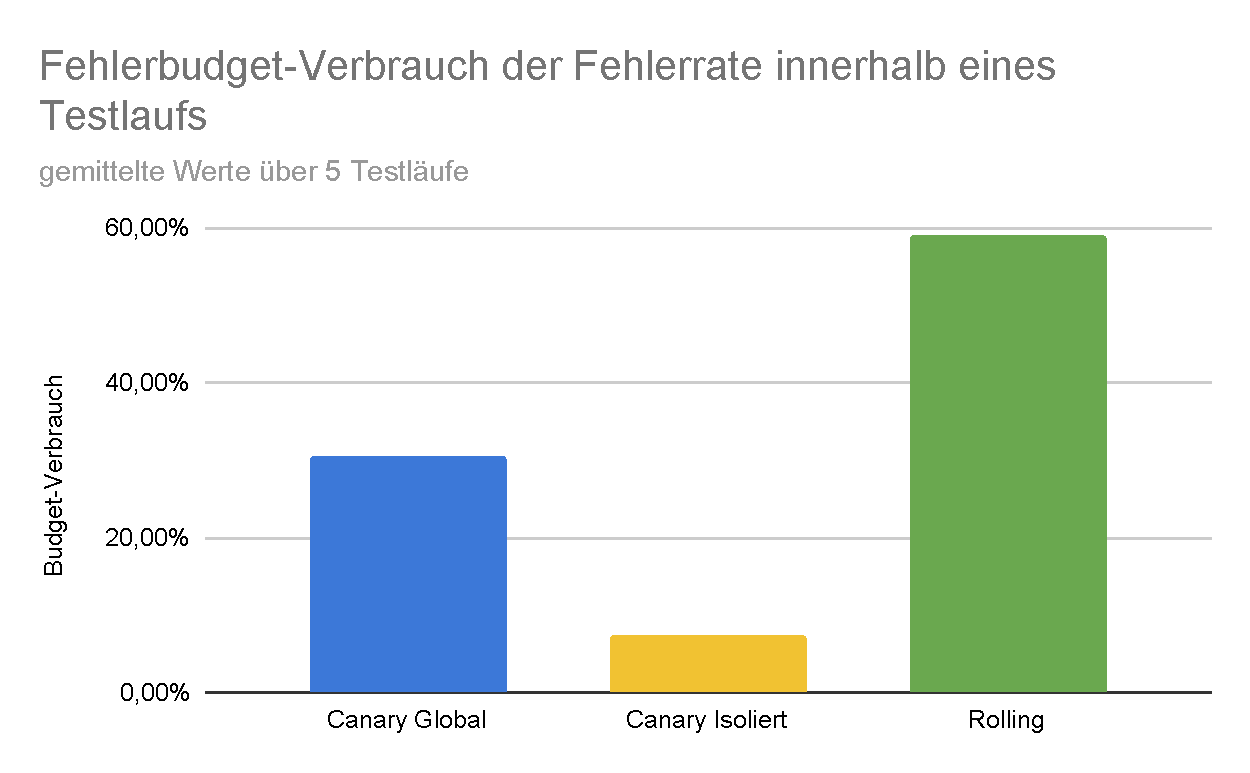
\includegraphics[width=0.8\textwidth]{images/eval-pdf/Fehlerbudget-Verbrauch der Fehlerrate innerhalb eines Testlaufs.pdf}
		\caption{Verbrauch des Fehlerbudgets unterschiedlicher Deployment Strategien bei injizierter Fehlerrate über die Testdauer}
		\label{fig:mid-budget-consumption-error-by-strategy}
	\end{figure} 

	\subsection{Fehlerszenario B}
	Abbildung \ref{fig:mid-budget-consumption-latenz-by-strategy} zeigt ebenfalls den Einfluss der Analysemetrik und Deployment Strategie hinsichtlich des Verbrauchs des Fehlerbudgets. Während der geringste Bedarf von 0,25\% am Fehlerbudget durch die isolierte Analysemetrik des Canary Releases erreicht wurde, verbrauchte die globale Analyse 2,59\%. Das Rolling Update stellte mit rund 26\% den höchsten Bedarf am Fehlerbudget. Die Einsparung des Fehlerbudgets von Canary Release mit globaler Analyse beläuft sich auf 23,4 Prozentpunkte gegenüber dem Rolling Update. Das Canary Release mit isolierter Analyse erreichte eine Einsparung von 25,74 Prozentpunkten gegenüber dem Rolling Update. Die Verringerung der Canary Release Strategie mit isolierter gegenüber globaler Analyse beläuft sich auf 2,34 Prozentpunkte.

	\begin{figure}[htbp]
		\centering
		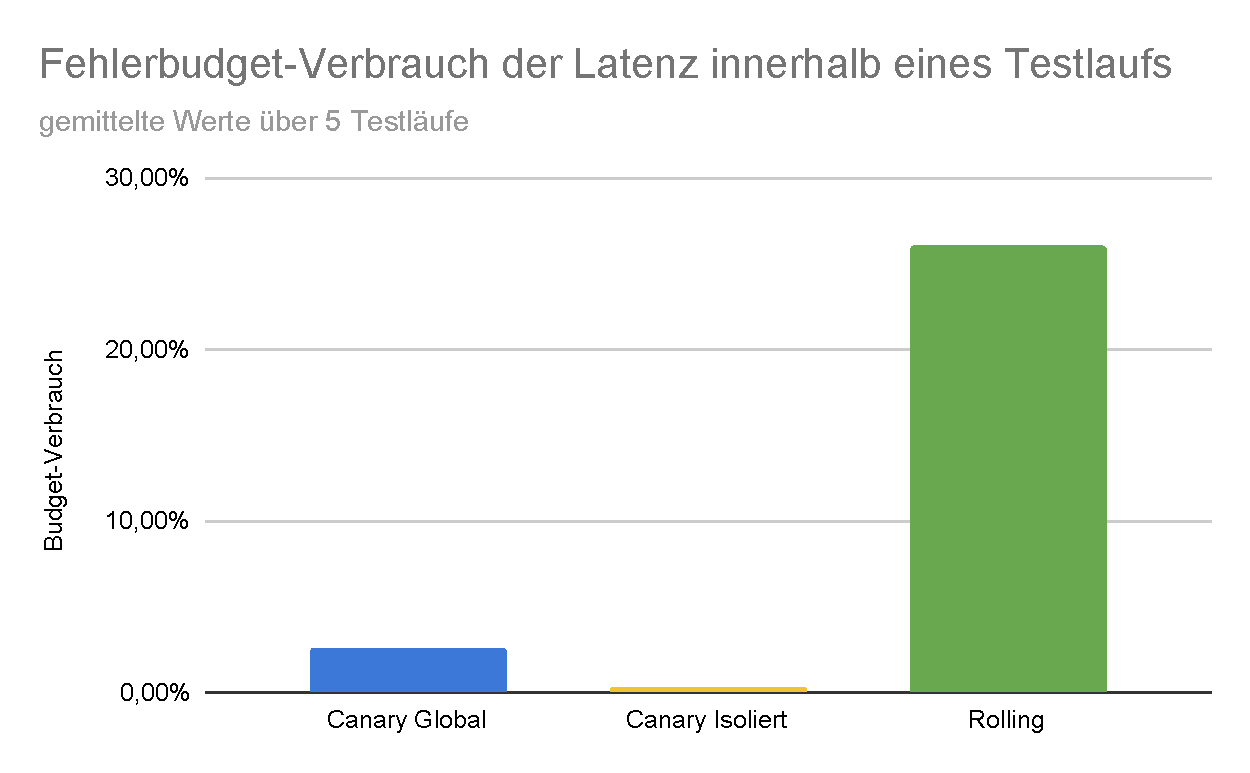
\includegraphics[width=0.8\textwidth]{images/eval-pdf/Fehlerbudget-Verbrauch der Latenz innerhalb eines Testlaufs.pdf}
		\caption{Verbrauch des Fehlerbudgets unterschiedlicher Deployment Strategien bei injizierter Latenz über die Testdauer}
		\label{fig:mid-budget-consumption-latenz-by-strategy}
	\end{figure} 
	
	\chapter{Diskussion}
	
	\section{Interpretation der Ergebnisse}
	
	\chapter{Fazit und Ausblick}
	
	\section{Beantwortung der Forschungsfrage}
	
	\section{Handlungsempfehlungen}
	
	
	% Literaturverzeichnis
	\printbibliography
	
	\appendix
	\chapter{Eigenständigkeitserklärung}
	Hiermit erkläre Ich, dass die vorliegende Arbeit selbstständig und nur unter Verwendung der angegebenen Literatur und Hilfsmittel angefertigt habe. Stellen, die wörtlich oder sinngemäß aus Quellen entnommen wurden, sind als solche kenntlich gemacht. Diese Arbeit wurde in gleicher oder ähnlicher Form noch keiner anderen Prüfungsbehörde vorgelegt.
	
	\vspace{2cm}
	
	\noindent
	%\makebox[6cm]{\hrulefill}
	\hfill
	\makebox[6cm]{\hrulefill}
	
	\noindent
	Borna, den 24.03.2026 	\hfill Paul Fuchs
	
\end{document}
